\flushbottom

%%
%% Add a graph to example 1.2.5, $\sign(x)$.
%%
%% Add a section on the inner product.  use some of the material in sug5.
%% Do vectors as an example.
%%




%%============================================================================
%%============================================================================
\chapter{Hilbert Spaces}





An expert is a man who has made all the mistakes which can be made, 
in a narrow field.

\begin{flushright}
  - Niels Bohr
\end{flushright}










%% CONTINUE
WARNING: UNDER HEAVY CONSTRUCTION.

In this chapter we will introduce Hilbert spaces.  We develop the two 
important examples: $l_2$, the space of square summable infinite vectors 
and $L_2$, the space of square integrable functions.







%% CONTINUE: this section may need some work
%%============================================================================
\section{Linear Spaces}
\index{linear space}


A \textit{linear space} is a set of elements $\{x, y, z, \ldots\}$
that is closed under addition and scalar multiplication.  By closed under 
addition we mean: if $x$ and $y$ are elements, then $z = x + y$ is an element.
The addition is commutative and associative.
\begin{gather*}
  x + y = y + x \\
  (x + y) + z = x + (y + z)
\end{gather*}
Scalar multiplication is associative and distributive.
Let $a$ and $b$ be scalars, $a,b \in \mathbb{C}$.
\begin{gather*}
  (a b) x = a (b x) \\
  (a + b) x = a x + b x \\
  a(x + y) = a x + a y
\end{gather*}

All the linear spaces that we will work with have additional properties:
The zero element $0$ is the additive identity.
\[
x + 0 = x
\]
Multiplication by the scalar $1$ is the multiplicative identity.
\[
1 x = x
\]
Each element $x$ and the additive inverse, $-x$.
\[
x + (-x) = 0
\]


Consider a set of elements $\{x_1, x_2, \ldots\}$.  Let the $c_i$ be scalars.
If 
\[
y = c_1 x_1 + c_2 x_2 + \cdots
\]
then $y$ is a \textit{linear combination} of the $x_i$.
A set of elements $\{x_1, x_2, \ldots\}$ is \textit{linearly independent} if 
the equation
\[
c_1 x_1 + c_2 x_2 + \cdots = 0
\]
has only the trivial solution $c_1 = c_2 = \cdots = 0$.  Otherwise the set
is \textit{linearly dependent}. 


Let $\{e_1, e_2, \cdots\}$ be a linearly independent set of elements.
If every element $x$ can be written as a linear combination of the $e_i$
then the set $\{ e_i \}$ is a \textit{basis} for the space.  
The $e_i$ are called \textit{base elements}.
\[
x = \sum_{i} c_i e_i
\]
The set $\{e_i\}$ is also called a \textit{coordinate system}.  The scalars
$c_i$ are the \textit{coordinates} or $\textit{components}$ of $x$.
If the set $\{e_i\}$ is a basis, then we say that the set is 
\textit{complete}.





%%\begin{Example}
%% CONTINUE: vectors
%%\end{Example}





%%\begin{Example}
%% CONTINUE: C^2 functions, 
%% C^2 functions which satisfy homogeneous or periodic boundary conditions
%% C^2 functions which satisfy inhom boundary conditions for a counter-example
%%\end{Example}












%% CONTINUE: this section may need some work
%%============================================================================
\section{Inner Products}


$\langle x | y \rangle$ is an \textit{inner product} of two elements $x$ and $y$ if it 
satisfies the properties:
\begin{enumerate}
  %%
\item
  Conjugate-commutative.
  \[
  \langle x | y \rangle = \overline{ \langle x | y \rangle }
  \]
  %%
\item
  Linearity in the second argument.
  \[
  \langle x | a y + b z \rangle = a \langle x | y \rangle + b \langle x | y \rangle
  \]
  %%
\item
  Positive definite.
  \begin{gather*}
    \langle x | x \rangle \geq 0 \\
    \langle x | x \rangle = 0\ \mathrm{if and only if}\ x = 0
  \end{gather*}
\end{enumerate}

From these properties one can derive the properties:
\begin{enumerate}
  %%
\item
  Conjugate linearity in the first argument.
  \[
  \langle a x + b y | z \rangle = \overline{a} \langle x | z \rangle + \overline{b} \langle x | z \rangle
  \]
  %%
\item
  Schwarz Inequality.
  \[
  \left| \langle x | y \rangle \right|^2 \leq \langle x | x \rangle \langle y | y \rangle
  \]
\end{enumerate}





One inner product of vectors is the \textit{Euclidean inner product}.
\[
\langle \mathbf{x} | \mathbf{y} \rangle \equiv \mathbf{x} \cdot \mathbf{y} = \sum_{i=0}^n \overline{x_i} y_i.
\]

One inner product of functions defined on $(a \ldots b)$ is
\[
\langle u | v \rangle = \int_a^b \overline{u(x)} v(x) \,\dd x.
\]
If $\sigma(x)$ is a positive-valued function, then we can define the
inner product:
\[
\langle u | \sigma| v \rangle = \int_a^b \overline{u(x)} \sigma(x) v(x) \,\dd x.
\]
This is called the inner product with respect to the weighting function 
$\sigma(x)$.  It is also denoted $\langle u | v \rangle_\sigma$.




%% CONTINUE: this section may need some work
%%============================================================================
\section{Norms}


A \textit{norm} is a real-valued function on a space which satisfies the
following properties.
\begin{enumerate}
\item
  Positive.
  \[
  \|x\| \geq 0
  \]
\item
  Definite.
  \[
  \|x\| = 0\ \mathrm{if and only if}\ x = 0
  \]
\item
  Multiplication my a scalar, $c \in \mathbb{C}$.
  \[
  \| c x \| = |c| \|x \|
  \]
\item
  Triangle inequality.
  \[
  \|x + y\| \leq \|x\| + \|y\|
  \]
\end{enumerate}




\begin{Example}
  Consider a vector space, (finite or infinite dimension), with elements
  $x = (x_1, x_2, x_3, \ldots)$.  Here are some common norms.
  \begin{itemize}
  \item
    Norm generated by the inner product.
    \[
    \|x\| = \sqrt{\langle x | x \rangle}
    \]
  \item
    The $l_p$ norm.
    \[
    \|x\|_p = \left( \sum_{k = 1}^\infty |x_k|^p \right)^{1/p}
    \]
    There are three common cases of the $l_p$ norm.
    \begin{itemize}
    \item
      Euclidian norm, or $l_2$ norm.
      \[
      \|x\|_2 = \sqrt{ \sum_{k = 1}^\infty |x_k|^2 }
      \]
    \item
      $l_1$ norm.
      \[
      \|x\|_1 = \sum_{k = 1}^\infty |x_k|
      \]
    \item
      $l_\infty$ norm.
      \[
      \|x\|_\infty = \max_k |x_k|
      \]
    \end{itemize}
  \end{itemize}
\end{Example}






\begin{Example}
  Consider a space of functions defined on the interval $(a \ldots b)$.
  Here are some common norms.
  \begin{itemize}
  \item
    Norm generated by the inner product.
    \[
    \|u\| = \sqrt{\langle u | u \rangle}
    \]
  \item
    The $L_p$ norm.
    \[
    \|u\|_p = \left( \int_a^b |u(x)|^p \,\dd x \right)^{1/p}
    \]
    There are three common cases of the $L_p$ norm.
    \begin{itemize}
    \item
      Euclidian norm, or $L_2$ norm.
      \[
      \|u\|_2 = \sqrt{ \int_a^b |u(x)|^2 \,\dd x }
      \]
    \item
      $L_1$ norm.
      \[
      \|u\|_1 = \int_a^b |u(x)| \,\dd x
      \]
    \item
      $L_\infty$ norm.
      \[
      \|u\|_\infty = \limsup_{x \in (a \ldots b)} |u(x)|
      \]
    \end{itemize}
  \end{itemize}
\end{Example}




%% CONTINUE


\paragraph{Distance.}
Using the norm, we can define the distance between elements $u$ and $v$.
\[
d(u,v) \equiv \|u - v \|
\]
Note that $d(u,v) = 0$ does not necessarily imply that $u = v$.
CONTINUE.



%% CONTINUE: Write
%%============================================================================
\section{Linear Independence.}

%%Define linear independence, span, etc.
%%Cover projections onto a subspace.
%%project sin(x) onto the space {1,x,...,x^n}
%%CONTINUE.




%% CONTINUE: Write
%%============================================================================
\section{Orthogonality}

%%Show how orthogonality is better than linear independence.
%%CONTINUE.

Orthogonality.
\[
\langle \phi_j | \phi_k \rangle = 0\ \mathrm{if}\ j \neq k
\]

Orthonormality.
\[
\langle \phi_j | \phi_k \rangle = \delta_{j k}
\]



\begin{Example}
  Infinite vectors.
  $e_j$ has all zeros except for a 1 in the $j^{\mathrm{th}}$ position. 
  \[
  e_j = (0, 0, \ldots 0, 1, 0, \ldots)
  \]
  %% CONTINUE HERE
\end{Example}



\begin{Example}
  $L_2$ functions on $(0 \ldots 2 \pi)$.
  \[
  \phi_j = \frac{1}{\sqrt{2\pi}} \e^{\imath j x}, \quad j \in \mathbb{Z}
  \]
  \[
  \phi_0 = \frac{1}{\sqrt{2\pi}}, \quad
  \phi_j^{(1)} = \frac{1}{\sqrt{\pi}} \cos(j x), \quad
  \phi_j^{(1)} = \frac{1}{\sqrt{\pi}} \sin(j x), \quad j \in \mathbb{Z}^+
  \]
  %% CONTINUE HERE
\end{Example}



%%The sine series is complete on (0...\pi), but not on (-\pi...\pi).
%% CONTINUE HERE





%% CONTINUE HERE




%%============================================================================
\section{Gramm-Schmidt Orthogonalization}
\index{Gramm-Schmidt orthogonalization}

Let $\{\psi_1(x), \ldots, \psi_n(x)\}$ be a set of linearly independent 
functions.  Using the Gramm-Schmidt orthogonalization process we can
construct a set of orthogonal functions $\{\phi_1(x), \ldots, \phi_n(x)\}$
that has the same span as the set of $\psi_n$'s with the formulas
\begin{align*}
  \phi_1 &= \psi_1 \\
  \phi_2 &= \psi_2 - \frac{\langle \phi_1 | \psi_2 \rangle}{\|\phi_1\|^2} \phi_1\\
  \phi_3 &= \psi_3 - \frac{\langle \phi_1 | \psi_3 \rangle}{\|\phi_1\|^2} \phi_1 
  - \frac{\langle \phi_2 | \psi_3 \rangle}{\|\phi_2\|^2} \phi_2\\
  \cdots & \\
  \phi_n &= \psi_n - \sum_{j=1}^{n-1} \frac{\langle \phi_j | \psi_n \rangle}
  {\|\phi_j\|^2} \phi_j.
\end{align*}

You could verify that the $\phi_m$ are orthogonal with a proof by induction.




\begin{Example}
  Suppose we would like a polynomial approximation to $\cos(\pi x)$ in the
  domain $[-1,1]$.  One way to do this is to find the Taylor expansion of 
  the function about $x=0$.  Up to terms of order $x^4$, this is
  \[ 
  \cos(\pi x) = 1 - \frac{(\pi x)^2}{2} + \frac{(\pi x)^4}{24} + O(x^6).
  \]
  In the first graph of Figure~\ref{least_cos} $\cos(\pi x)$ and this fourth 
  degree polynomial are plotted.
  We see that the approximation is very good near $x=0$, but deteriorates
  as we move away from that point.  This makes sense because the Taylor
  expansion only makes use of information about the function's behavior
  at the point $x=0$.

  As a second approach, we could find the least squares fit of a fourth
  degree polynomial to $\cos(\pi x)$.  The set of functions
  $\{1, x, x^2, x^3, x^4\}$ is independent, but not orthogonal in the interval
  $[-1,1]$.  Using Gramm-Schmidt orthogonalization,
  \begin{align*}
    \phi_0 &= 1 \\
    \phi_1 &= x - \frac{\langle 1 | x \rangle}{\langle 1 | 1 \rangle} = x \\
    \phi_2 &= x^2 - \frac{\langle 1 | x^2 \rangle}{\langle 1 | 1 \rangle}
    - \frac{\langle x | x^2 \rangle}{\langle x | x \rangle}x = x^2 - \frac{1}{3} \\
    \phi_3 &= x^3 - \frac{3}{5} x \\
    \phi_4 &= x^4 - \frac{6}{7}x^2 - \frac{3}{35}
  \end{align*}
  A widely used set of functions in mathematics is the set of 
  \textbf{Legendre polynomials} $\{P_0(x), P_1(x), \ldots\}$.
  \index{Legendre polynomials}
  They differ from the $\phi_n$'s that we generated only by constant factors.
  The first few are
  \begin{align*}
    P_0(x) &= 1 \\
    P_1(x) &= x \\
    P_2(x) &= \frac{3x^2 - 1}{2} \\
    P_3(x) &= \frac{5x^3 - 3x}{2} \\
    P_4(x) &= \frac{35x^4 - 30x^2 + 3}{8}.
  \end{align*}

  Expanding $\cos(\pi x)$ in Legendre polynomials
  \[ \cos(\pi x) \approx \sum_{n=0}^4 c_n P_n(x), \]
  and calculating the generalized Fourier coefficients with the formula
  \[ c_n = \frac{\langle P_n | \cos(\pi x) \rangle}{\langle P_n | P_n \rangle}, \]
  yields 
  \begin{align*}
    \cos(\pi x) &\approx - \frac{15}{\pi^2} P_2(x) + \frac{45(2\pi^2-21)}{\pi^4}
    P_4(x) \\
    &= \frac{105}{8\pi^4} [(315-30\pi^2)x^4 + (24\pi^2 - 270)x^2 + 
    (27 - 2\pi^2)]
  \end{align*}
  The cosine and this polynomial are plotted in the second graph in
  Figure~\ref{least_cos}.  The least squares fit method uses information
  about the function on the entire interval.  We see that the least
  squares fit does not give as good an approximation close to the
  point $x=0$ as the Taylor expansion.  However, the least squares fit gives a
  good approximation on the entire interval.  

  In order to expand a function in a Taylor series, the function must be analytic
  in some domain.  One advantage of using the method of least squares is that the
  function being approximated does not even have to be continuous.

  \begin{figure}[h!]
    \begin{center}
      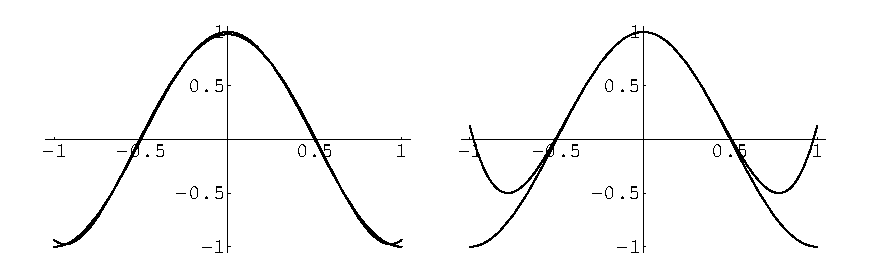
\includegraphics[width=\textwidth]{ode/hilbert/least}
    \end{center}
    \caption{Polynomial approximations of the function.}
    \label{least_cos}
  \end{figure}


\end{Example}





%% CONTINUE: Complete this.
%%============================================================================
\section{Orthonormal Function Expansion}

Let $\{\phi_j\}$ be an orthonormal set of functions
on the interval $(a,b)$.  We expand a function $f(x)$ in the $\phi_j$.
\[
f(x) = \sum_j c_j \phi_j
\]
We choose the coefficients to minimize the norm of the error.
\begin{align*}
  \left\| f - \sum_j c_j \phi_j \right\|^2 
  &= \left\langle f - \sum_j c_j \phi_j \bigg| 
    f - \sum_j c_j \phi_j \right\rangle \\
  &= \| f \|^2 
  - \left\langle f \bigg| \sum_j c_j \phi_j \right\rangle
  - \left\langle \sum_j c_j \phi_j \bigg| f \right\rangle
  + \left\langle \sum_j c_j \phi_j \bigg| 
    \sum_j c_j \phi_j \right\rangle \\
  &= \| f \|^2 + \sum_j |c_j|^2
  - \sum_j c_j \langle f | \phi_j \rangle
  - \sum_j \overline{c_j} \langle \phi_j | f \rangle 
\end{align*}
\begin{equation}
  \label{eqn_f2_sjcjpjf}
  \left\| f - \sum_j c_j \phi_j \right\|^2 
  = \| f \|^2 + \sum_j |c_j|^2
  - \sum_j c_j \overline{\langle \phi_j | f \rangle}
  - \sum_j \overline{c_j} \langle \phi_j | f \rangle
\end{equation}
To complete the square, we add the constant 
$\sum_j \langle \phi_j | f \rangle \overline{ \langle \phi_j | f \rangle }$.
We see the values of $c_j$ which minimize
\[
\| f \|^2 + \sum_j \left| c_j - \langle \phi_j | f \rangle \right|^2.
\]
Clearly the unique minimum occurs for
\[
c_j = \langle \phi_j | f \rangle.
\]
We substitute this value for $c_j$ into the right side of 
Equation~\ref{eqn_f2_sjcjpjf} and note that this quantity, the squared norm
of the error, is non-negative.
\begin{gather*}
  \| f \|^2 + \sum_j |c_j|^2 - \sum_j |c_j|^2 - \sum_j |c_j|^2 \geq 0 \\
  \| f \|^2 \geq \sum_j |c_j|^2 
\end{gather*}
This is known as \textit{Bessel's Inequality}.  If the set of $\{\phi_j\}$ is 
complete then the norm of the error is zero and we obtain 
\textit{Bessel's Equality}.
\[
\| f \|^2 = \sum_j |c_j|^2 
\]
%% CONTINUE HERE: unitary transformations, Parseval's relation.






%% CONTINUE: slice this up and fold it into the chapter.
%%============================================================================
\section{Sets Of Functions}

\paragraph{Orthogonality.}
Consider two complex valued functions of a real variable
$\phi_1(x)$ and $\phi_2(x)$ defined
on the interval $a \leq x \leq b$.  The inner product of the two functions
is defined
\index{inner product!of functions}
\[ \langle \phi_1 | \phi_2 \rangle = \int_a^b \overline{\phi_1}(x) \phi_2(x)\,\dd x.\]
The two functions are orthogonal if $\langle \phi_1 | \phi_2 \rangle = 0$.  The $L_2$
norm of a function is defined $\| \phi \| = \sqrt{\langle \phi | \phi \rangle}$.
\index{norm!of functions}

Let $\{ \phi_1, \phi_2, \phi_3, \ldots\}$ be a set of complex valued
functions.  The set of functions is orthogonal if each pair of functions
is orthogonal.  That is,
\[ \langle \phi_n | \phi_m \rangle = 0 \quad \mathrm{if}\ n \neq m.\]
If in addition the norm of each function is $1$, then the set is orthonormal.
\index{orthonormal}
That is,
\[ \langle \phi_n | \phi_m \rangle = \delta_{nm} = 
\begin{cases}
  1 \quad &\mathrm{if}\ n = m \\
  0 \quad &\mathrm{if}\ n \neq m.
\end{cases}
\]


\begin{Example}
  The set of functions
  \[ \left\{ \sqrt{\frac{2}{\pi}} \sin(x), \sqrt{\frac{2}{\pi}} \sin(2 x),
    \sqrt{\frac{2}{\pi}} \sin(3 x), \ldots \right\} \]
  is orthonormal on the interval $[0, \pi]$.
  To verify this,
  \begin{align*}
    \left\langle \sqrt{\frac{2}{\pi}} \sin(n x) \Bigg| 
      \sqrt{\frac{2}{\pi}} \sin(n x) \right\rangle
    &= \frac{2}{\pi} \int_0^\pi \sin^2(n x)\,\dd x \\
    &= 1
  \end{align*}
  If $n \neq m$ then
  \begin{align*}
    \left\langle \sqrt{\frac{2}{\pi}} \sin(n x) \Bigg| 
      \sqrt{\frac{2}{\pi}} \sin(m x) \right\rangle
    &= \frac{2}{\pi} \int_0^\pi \sin(n x) \sin(m x)\,\dd x \\
    &= \frac{1}{\pi} \int_0^\pi (\cos[(n-m)x] - \cos[(n+m)x])\,\dd x \\
    &= 0.
  \end{align*}
\end{Example}








\begin{Example}
  The set of functions
  \[ \{ \ldots, \frac{1}{\sqrt{2\pi}} \e^{-\imath x}, \frac{1}{\sqrt{2\pi}}, 
  \frac{1}{\sqrt{2\pi}} \e^{\imath x}, \frac{1}{\sqrt{2\pi}} \e^{\imath 2 x},
  \ldots \}, \]
  is orthonormal on the interval $[-\pi, \pi]$.
  To verify this,
  \begin{align*}
    \left\langle \frac{1}{\sqrt{2\pi}} \e^{\imath n x} \Bigg| \frac{1}{\sqrt{2\pi}}
      \e^{\imath n x} \right\rangle
    &= \frac{1}{2\pi} \int_{-\pi}^\pi \e^{-\imath n x} \e^{\imath n x}\,\dd x \\
    &= \frac{1}{2\pi} \int_{-\pi}^\pi \,\dd x \\
    &= 1.
  \end{align*}
  If $n \neq m$ then
  \begin{align*}
    \left\langle \frac{1}{\sqrt{2\pi}} \e^{\imath n x} \Bigg| \frac{1}{\sqrt{2\pi}}
      \e^{\imath m x} \right\rangle
    &= \frac{1}{2\pi} \int_{-\pi}^\pi \e^{-\imath n x} \e^{\imath m x}\,\dd x \\
    &= \frac{1}{2\pi} \int_{-\pi}^\pi \e^{\imath (m - n) x}\,\dd x \\
    &= 0.
  \end{align*} 
\end{Example}














\paragraph{Orthogonal with Respect to a Weighting Function.}
\index{orthogonality!weighting functions}

Let $\sigma(x)$ be a real-valued, positive function on the 
interval $[a,b]$.  We introduce the notation
\[ \langle \phi_n | \sigma | \phi_m \rangle \equiv \int_a^b \overline{\phi_n}
\sigma \phi_m\, d x.\]
If the set of functions $\{\phi_1, \phi_2, \phi_3, \ldots\}$ satisfy 
\[ \langle \phi_n | \sigma | \phi_m \rangle = 0 \quad \mathrm{if}\ n \neq m \]
then the functions are orthogonal with respect to the weighting function
$\sigma(x)$. 

If the functions satisfy
\[ \langle \phi_n | \sigma | \phi_m \rangle = \delta_{nm} \]
then the set is orthonormal with respect to $\sigma(x)$.



\begin{Example}
  We know that the set of functions
  \[ \left\{ \sqrt{\frac{2}{\pi}} \sin(x), \sqrt{\frac{2}{\pi}} \sin(2 x),
    \sqrt{\frac{2}{\pi}} \sin(3 x), \ldots \right\} \]
  is orthonormal on the interval $[0, \pi]$.
  That is,
  \[ \int_0^\pi \sqrt{\frac{2}{\pi}} \sin(n x) 
  \sqrt{\frac{2}{\pi}} \sin(m x) \,\dd x = \delta_{nm}. \]
  If we make the change of variables $x = \sqrt{t}$ in this integral, we obtain
  \[ \int_0^{\pi^2} \frac{1}{2\sqrt{t}} \sqrt{\frac{2}{\pi}} \sin(n \sqrt{t})
  \sqrt{\frac{2}{\pi}} \sin(m \sqrt{t})\, d t = \delta_{nm}.\]
  Thus the set of functions
  \[ \left\{ \sqrt{\frac{1}{\pi}} \sin(\sqrt{t}), \sqrt{\frac{1}{\pi}} \sin(2\sqrt{t}),
    \sqrt{\frac{1}{\pi}} \sin(3\sqrt{t}), \ldots \right\} \]
  is orthonormal with respect to $\sigma(t) = \frac{1}{2 \sqrt{t}}$ on the interval
  $[0, \pi^2]$.
\end{Example}







\paragraph{Orthogonal Series.}
\index{orthogonal series}
Suppose that a function $f(x)$ defined on $[a,b]$
can be written as a uniformly convergent sum of functions that are 
orthogonal with respect to $\sigma(x)$.
\[ f(x) = \sum_{n = 1}^\infty c_n \phi_n(x) \]
We can solve for the $c_n$ by taking the inner product of $\phi_m(x)$ and 
each side of the equation with respect to $\sigma(x)$. 
\begin{gather*}
  \langle \phi_m | \sigma | f \rangle = \left\langle \phi_m \Bigg| \sigma \Bigg| 
    \sum_{n = 1}^\infty c_n \phi_n \right\rangle \\
  \langle \phi_m | \sigma | f \rangle = \sum_{n = 1}^\infty c_n \langle \phi_m | \sigma | \phi_n 
  \rangle \\
  \langle \phi_m | \sigma | f \rangle = c_m \langle \phi_m | \sigma | \phi_m \rangle \\
  c_m = \frac{\langle \phi_m | \sigma | f \rangle}{\langle \phi_m  | \sigma | \phi_m \rangle}
\end{gather*}
The $c_m$ are known as \textbf{Generalized Fourier coefficients}.
\index{Fourier coefficients}
If the functions in the expansion are orthonormal, the formula simplifies
to
\[ c_m = \langle \phi_m | \sigma | f \rangle. \]














\begin{Example}
  The function $f(x) = x(\pi - x)$ has a uniformly convergent series
  expansion in the domain $[0,\pi]$ of the form
  \[ x(\pi - x) = \sum_{n = 1}^\infty c_n \sqrt{\frac{2}{\pi}} \sin(n x).\]
  The Fourier coefficients are
  \begin{align*}
    c_n     &= \left\langle \sqrt{\frac{2}{\pi}} \sin(n x) \Bigg| x(\pi-x) \right\rangle \\
    &= \sqrt{\frac{2}{\pi}} \int_0^\pi x(\pi-x) \sin(n x)\,\dd x \\
    &= \sqrt{\frac{2}{\pi}} \frac{2}{n^3} (1 - (-1)^n) \\
    &= 
    \begin{cases}
      \sqrt{\frac{2}{\pi}} \frac{4}{n^3} \quad &\mathrm{for odd}\ n \\
      0 \quad &\mathrm{for even}\ n
    \end{cases}
  \end{align*}
  Thus the expansion is
  \[ x(\pi-x) = \sum_{\substack{ {n} = 1 \\ \mathrm{odd}\ n}}^{\infty} \frac{8}{\pi n^3} \sin(n x) \quad \mathrm{for}\ x \in [0, \pi]. \]

  In the first graph of Figure~\ref{sin_par} the first term in the expansion
  is plotted in a dashed line and $x (\pi - x)$ is plotted in a solid line.
  The second graph shows the two term approximation.

  \begin{figure}[h!]
    \begin{center}
      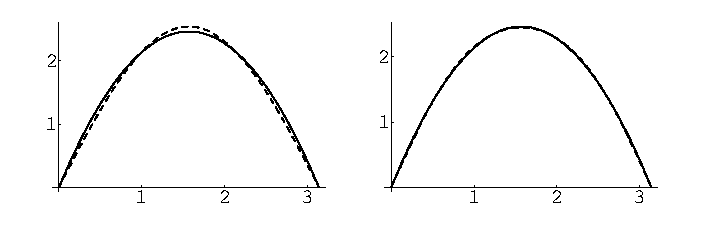
\includegraphics[width=\textwidth]{ode/hilbert/sin_par}
    \end{center}
    \caption{Series expansions of the function.}
    \label{sin_par}
  \end{figure}

\end{Example}












\begin{Example}
  The set $\{ \ldots, 1/\sqrt{2\pi} \e^{-\imath x}, 1/\sqrt{2\pi}, 
  1/\sqrt{2\pi} \e^{\imath x}, 1/\sqrt{2\pi} \e^{\imath 2 x}, \ldots\}$ is orthonormal
  on the interval $[-\pi,\pi]$.  $f(x) = \sign(x)$ has the
  expansion
  \begin{align*}
    \sign(x) 
    &\sim \sum_{n = -\infty}^\infty \left\langle \frac{1}{\sqrt{2\pi}} \e^{\imath n \xi} \Bigg| \sign(\xi) \right\rangle
    \frac{1}{\sqrt{2\pi}} \e^{\imath n x} \\
    &= \frac{1}{2\pi} \sum_{n = -\infty}^\infty \int_{-\pi}^\pi \e^{-\imath n \xi} \sign(\xi)
    \,\dd \xi \e^{\imath n x} \\
    &= \frac{1}{2\pi} \sum_{n = -\infty}^\infty \left( \int_{-\pi}^0 - \e^{-\imath n \xi}\,\dd \xi
      + \int_0^\pi \e^{-\imath n \xi}\,\dd \xi \right)
    \e^{\imath n x} \\
    &= \frac{1}{\pi} \sum_{n = -\infty}^\infty \frac{1 - (-1)^n}{\imath n} \e^{\imath n x}. \\
    \intertext{In terms of real functions, this is}
    &= \frac{1}{\pi} \sum_{n = -\infty}^\infty \frac{1 - (-1)^n}{\imath n} 
    (\cos(n x) + \imath \sin(n x)) \\
    &= \frac{2}{\pi} \sum_{n = 1}^\infty \frac{1 - (-1)^n}{\imath n} \sin(n x) 
  \end{align*}
  \[ \boxed{ \sign(x) \sim \frac{4}{\pi} \sum_{\substack{ {n} = 1 \\ \mathrm{odd}\ n}}^{\infty} 
    \frac{1}{n} \sin(n x).} \]
\end{Example}







%% CONTINUE: slice this up and fold it into the chapter.
%%============================================================================
\section{Least Squares Fit to a Function and Completeness}

Let $\{\phi_1, \phi_2, \phi_3, \ldots \}$ be a set of real, square integrable
functions that are orthonormal with respect to the weighting function
$\sigma(x)$ on the interval $[a, b]$.  That is,
\[ \langle \phi_n | \sigma | \phi_m \rangle = \delta_{nm}. \]
Let $f(x)$ be some square integrable function defined on the same interval.
We would like to approximate the function $f(x)$ with a finite
orthonormal series.
\[ 
f(x) \approx \sum_{n=1}^N \alpha_n \phi_n(x) 
\]
$f(x)$ may or may not have a uniformly convergent expansion in the orthonormal
functions.

We would like to choose the $\alpha_n$ so that we get the best possible
approximation to $f(x)$.  The most common measure of how well a series
approximates a function is the least squares measure.  The error 
is defined as the integral of the weighting function times the 
square of the deviation.
\[ 
E = \int_a^b \sigma(x) \left( f(x) - \sum_{n=1}^N \alpha_n \phi_n(x) \right)^2\,\dd x 
\]
The ``best'' fit is found by choosing the $\alpha_n$ that minimize $E$.
Let $c_n$ be the Fourier coefficients of $f(x)$.
\[ 
c_n = \langle \phi_n | \sigma | f \rangle
\]
we expand the integral for $E$.
\begin{align*}
  E(\alpha)
  &= \int_a^b \sigma(x) \left( f(x) - \sum_{n=1}^N \alpha_n \phi_n(x) \right)^2\,\dd x 
  \\
  &= \biggl\langle f - \sum_{n=1}^N \alpha_n \phi_n \biggm| \sigma \biggm|
  f - \sum_{n=1}^N \alpha_n \phi_n \biggr\rangle 
  \\
  &= \langle f | \sigma | f \rangle 
  - 2 \bigg\langle \sum_{n=1}^N \alpha_n \phi_n \bigg| \sigma \bigg| f \bigg\rangle
  + \bigg\langle \sum_{n=1}^N \alpha_n \phi_n \bigg| \sigma \bigg| 
  \sum_{n=1}^N \alpha_n \phi_n \bigg\rangle 
  \\
  &= \langle f | \sigma | f \rangle 
  -2 \sum_{n=1}^N \alpha_n \langle \phi_n | \sigma | f \rangle
  + \sum_{n=1}^N \sum_{m=1}^N \alpha_n \alpha_m \langle \phi_n | \sigma | \phi_m \rangle 
  \\
  &= \langle f | \sigma | f \rangle - 2 \sum_{n=1}^N \alpha_n c_n
  + \sum_{n=1}^N \alpha_n^2 
  \\
  &= \langle f | \sigma | f \rangle + \sum_{n=1}^N (\alpha_n - c_n)^2 - \sum_{n=1}^N c_n^2
\end{align*}
Each term involving $\alpha_n$ in non-negative and is minimized for $\alpha_n = c_n$.
The Fourier coefficients give the least squares approximation to a function.
The least squares fit to $f(x)$ is thus
\[ 
f(x) \approx \sum_{n=1}^N \langle \phi_n | \sigma | f \rangle\, \phi_n(x). \]


\begin{Result}
  If $\{\phi_1, \phi_2, \phi_3, \ldots\}$ is a set of real, square integrable
  functions that are orthogonal with respect to $\sigma(x)$
  then the least squares fit of the first $N$ 
  orthogonal functions to the square integrable function $f(x)$ is
  \[ 
  f(x) \approx \sum_{n=1}^N \frac{\langle \phi_n | \sigma | f \rangle}
  {\langle \phi_n | \sigma | \phi_n \rangle} \phi_n(x).
  \]
  If the set is orthonormal, this formula reduces to
  \[ 
  f(x) \approx \sum_{n=1}^N \langle \phi_n | \sigma | f  \rangle\, \phi_n(x).
  \]
\end{Result}



Since the error in the approximation $E$ is a nonnegative number we can
obtain on inequality on the sum of the squared coefficients.
\begin{gather*}
  E = \langle f | \sigma | f \rangle - \sum_{n=1}^N c_n^2 \\
  \boxed{ \sum_{n=1}^N c_n^2 \leq \langle f | \sigma | f \rangle }
\end{gather*}
This equation is known as \textbf{Bessel's Inequality}.
\index{Bessel's Inequality}
Since $\langle f | \sigma | f \rangle$ is just a nonnegative number, independent
of $N$, the sum $\sum_{n = 1}^\infty c_n^2$ is convergent and $c_n \to 0$ as 
$n \to \infty$

\paragraph{Convergence in the Mean.}
\index{convergence!in the mean}
If the error $E$ goes to zero as $N$ tends to infinity
\[ 
\lim_{N \to \infty} \int_a^b \sigma(x) \left( f(x) - \sum_{n=1}^N c_n \phi_n(x) \right)^2 \, d x = 0,
\]
then the sum converges in the mean to $f(x)$ relative to the weighting 
function $\sigma(x)$.  This implies that
\begin{gather*}
  \lim_{N \to \infty} \left( \langle f | \sigma | f \rangle - \sum_{n=1}^N c_n^2 \right) = 0 
  \\
  \boxed{
    \sum_{n = 1}^\infty c_n^2 = \langle f | \sigma | f \rangle.
    }
\end{gather*}
This is known as \textbf{Parseval's identity}.

\paragraph{Completeness.}
\index{completeness!of sets of functions}
Consider a set of functions $\{ \phi_1, \phi_2, \phi_3, \ldots\}$ that is
orthogonal with respect to the weighting function $\sigma(x)$.
If every function $f(x)$ that is square integrable with respect to
$\sigma(x)$ has an orthogonal series expansion
\[ f(x) \sim \sum_{n = 1}^\infty c_n \phi_n(x) \]
that converges in the mean to $f(x)$, then the set is \textbf{complete}.






%%============================================================================
\section{Closure Relation}
\index{closure relation!discrete sets of functions}

Let $\{ \phi_1, \phi_2, \ldots \}$ be an orthonormal, complete set on the
domain $[a,b]$.  For any
square integrable function $f(x)$ we can write
\[ f(x) \sim \sum_{n = 1}^\infty c_n \phi_n(x).\]
Here the $c_n$ are the generalized Fourier coefficients and the sum converges
in the mean to $f(x)$.  Substituting the expression for the Fourier
coefficients into the sum yields
\begin{align*}
  f(x) &\sim \sum_{n = 1}^\infty \langle \phi_n | f \rangle \phi_n(x) \\
  &= \sum_{n = 1}^\infty \left( \int_a^b \overline{\phi_n(\xi)} f(\xi)\,\dd \xi 
  \right) \phi_n(x). \\
  \intertext{Since the sum is not necessarily uniformly convergent, we are
    not justified in exchanging the order of summation and integration\ldots but
    what the heck, let's do it anyway.}
  &= \int_a^b \left(\sum_{n = 1}^\infty \overline{\phi_n(\xi)} f(\xi) \phi_n(x) 
  \right)\,\dd \xi \\
  &= \int_a^b \left(\sum_{n = 1}^\infty \overline{\phi_n(\xi)} \phi_n(x) \right)
  f(\xi)\,\dd \xi
\end{align*}

The sum behaves like a Dirac delta function.  
\index{Dirac delta function}
Recall that $\delta(x-\xi)$ satisfies the equation
\[ f(x) = \int_a^b \delta(x-\xi) f(\xi)\,\dd \xi \quad \mathrm{for}\ 
x \in (a,b). \]
Thus we could say that the sum is a representation of $\delta(x-\xi)$. 
Note that a series representation of the delta function could not be 
convergent, hence the necessity of throwing caution to the wind when we
interchanged the summation and integration in deriving the series.
The \textbf{closure relation} for an orthonormal, complete set states
\[ \sum_{n = 1}^\infty \phi_n(x) \overline{\phi_n(\xi)} \sim \delta(x-\xi). \]







Alternatively, you can derive the closure relation by computing the generalized 
Fourier coefficients of the delta function.
\[ \delta(x-\xi) \sim \sum_{n = 1}^\infty c_n \phi_n(x) \]
\begin{align*}
  c_n     &= \langle \phi_n | \delta(x-\xi) \rangle \\
  &= \int_a^b \overline{\phi_n(x)} \delta(x-\xi)\,\dd x \\
  &= \overline{\phi_n(\xi)}
\end{align*}
\[ \delta(x-\xi) \sim \sum_{n = 1}^\infty \phi_n(x) \overline{\phi_n(\xi)} \]





\begin{Result}
  If $\{\phi_1, \phi_2, \ldots \}$ is an orthogonal, complete set on the 
  domain $[a,b]$, then 
  \[ 
  \sum_{n = 1}^\infty \frac{\phi_n(x) \overline{\phi_n(\xi)}}{\|\phi_n\|^2} 
  \sim \delta(x-\xi).
  \]
  If the set is orthonormal, then
  \[ 
  \sum_{n = 1}^\infty \phi_n(x) \overline{\phi_n(\xi)} \sim \delta(x-\xi). 
  \]
\end{Result}






\begin{Example}
  The integral of the Dirac delta function is the Heaviside function.  On the
  interval $x \in (-\pi, \pi)$
  \[\int_{-\pi}^x \delta(t)\,\dd t = H(x) = 
  \begin{cases}
    1 \quad &\mathrm{for}\ 0 < x < \pi \\
    0 \quad &\mathrm{for}\ -\pi < x < 0.
  \end{cases}
  \]

  Consider the orthonormal, complete set $\{\ldots, \frac{1}{\sqrt{2\pi}}
  \e^{-\imath x}, \frac{1}{\sqrt{2\pi}}, \frac{1}{\sqrt{2\pi}}\e^{\imath x}, \ldots \}$ 
  on the domain $[-\pi,\pi]$.  The delta function has the series
  \[ \delta(t) \sim \sum_{n = -\infty}^\infty \frac{1}{\sqrt{2\pi}} \e^{\imath n t} 
  \frac{1}{\sqrt{2\pi}} \e^{-\imath n 0}
  = \frac{1}{2\pi} \sum_{n = -\infty}^\infty \e^{\imath n t}. \]

  We will find the series expansion of the Heaviside function
  first by expanding directly and then by integrating the expansion for
  the delta function.






  \paragraph{Finding the series expansion of $\mathbf{H(x)}$ directly.}
  The generalized Fourier coefficients of $H(x)$ are
  \begin{align*}
    c_0     &= \int_{-\pi}^\pi \frac{1}{\sqrt{2\pi}} H(x)\,\dd x \\
    &= \frac{1}{\sqrt{2\pi}} \int_0^\pi \,\dd x \\
    &= \sqrt{\frac{\pi}{2}} \\
    c_n     &= \int_{-\pi}^\pi \frac{1}{\sqrt{2\pi}} \e^{-\imath n x} H(x)\,\dd x \\
    &= \frac{1}{\sqrt{2\pi}} \int_0^\pi \e^{-\imath n x} \,\dd x \\
    &= \frac{1 - (-1)^n}{\imath n \sqrt{2\pi}}.
  \end{align*}
  Thus the Heaviside function has the expansion
  \begin{align*}
    H(x)    &\sim \sqrt{\frac{\pi}{2}} \frac{1}{\sqrt{2\pi}}
    + \sum_{\substack{ n = -\infty \\ n \neq 0 }}^\infty
    \frac{1 - (-1)^n}{\imath n \sqrt{2\pi}}
    \frac{1}{\sqrt{2\pi}} \e^{\imath n x} \\
    &= \frac{1}{2} + \frac{1}{\pi} \sum_{n = 1}^\infty \frac{1 - (-1)^n}{n}
    \sin(n x)
  \end{align*}
  \[ \boxed{H(x) \sim \frac{1}{2} + \frac{2}{\pi} \sum_{\substack{ {n} = 1 \\ \mathrm{odd}\ n}}^{\infty} 
    \frac{1}{n} \sin(n x).} \]





  \paragraph{Integrating the series for $\mathbf{\boldsymbol{\delta}(t)}$.}
  \begin{align*}
    \int_{-\pi}^x \delta(t)\,\dd t
    &\sim \frac{1}{2\pi} \int_{-\pi}^x \sum_{n = -\infty}^\infty \e^{\imath n t} \,\dd t \\
    &= \frac{1}{2\pi} \left( (x+\pi) + 
      \sum_{\substack{ n=-\infty \\ n \neq 0 }}^\infty
      \left[ \frac{1}{in}\e^{\imath n t} \right]_{-\pi}^x \right) \\
    &= \frac{1}{2\pi} \left( (x+\pi) + 
      \sum_{\substack{ n=-\infty \\ n \neq 0 }}^\infty
      \frac{1}{\imath n} \big(\e^{\imath n x} - (-1)^n\big) \right) \\
    &= \frac{x}{2\pi} + \frac{1}{2} + \frac{1}{2\pi}
    \sum_{n = 1}^\infty \frac{1}{\imath n} \big(\e^{\imath n x} - \e^{-\imath n x} 
    -(-1)^n + (-1)^n\big) \\
    &= \frac{x}{2\pi} + \frac{1}{2} + \frac{1}{\pi}
    \sum_{n = 1}^\infty \frac{1}{n} \sin(n x) 
  \end{align*}

  Expanding $\frac{x}{2\pi}$ in the orthonormal set,
  \[ \frac{x}{2\pi} \sim \sum_{n = -\infty}^\infty c_n \frac{1}{\sqrt{2\pi}} \e^{\imath n x}.\]
  \begin{align*}
    c_0     &= \int_{-\pi}^\pi \frac{1}{\sqrt{2\pi}} \frac{x}{2\pi}\,\dd x = 0 \\
    c_n     &= \int_{-\pi}^\pi \frac{1}{\sqrt{2\pi}} \e^{- \imath n x} 
    \frac{x}{2\pi}\,\dd x = \frac{\imath (-1)^n}{n \sqrt{2\pi}}
  \end{align*}
  \[
  \frac{x}{2\pi} \sim \sum_{\substack{ n=-\infty \\ n \neq 0 }}^\infty
  \frac{\imath (-1)^n}{n \sqrt{2\pi}} \frac{1}{\sqrt{2\pi}} \e^{\imath n x} 
  = -\frac{1}{\pi} \sum_{n = 1}^\infty (-1)^n \sin(n x)
  \]

  Substituting the series for $\frac{x}{2\pi}$ into the expression for
  the integral of the delta function,
  \[ \int_{-\pi}^x \delta(t)\,\dd t \sim \frac{1}{2} + \frac{1}{\pi} 
  \sum_{n = 1}^\infty \frac{1-(-1)^n}{n} \sin(n x) \]
  \[ \boxed{ \int_{-\pi}^x \delta(t)\,\dd t \sim \frac{1}{2} 
    + \frac{2}{\pi} \sum_{\substack{ {n} = 1 \\ \mathrm{odd}\ n}}^{\infty} \frac{1}{n}\sin(n x).} \]




  Thus we see that the series expansions of the Heaviside function and
  the integral of the delta function are the same.
\end{Example}






%% CONTINUE: this section may need some work
%%============================================================================
\section{Linear Operators}



%% CONTINUE











\raggedbottom
%%============================================================================
\exercises{
\pagebreak
\flushbottom
\section{Exercises}





%%-----------------------------------------------------------------------------
%%\begin{large}
%%\noindent
%%\textbf{}
%%\end{large}




%% Suppose $\{ \phi_k(x) \}_{k=0}^\infty$ is an orthogonal system on $[a,b]$.
\begin{Exercise}
  \label{exercise phik orthonormal}
  \begin{enumerate}
    %%
    %%
  \item
    Suppose $\{ \phi_k(x) \}_{k=0}^\infty$ is an orthogonal system on $[a,b]$.
    Show that any finite set of the $\phi_j(x)$ is a linearly independent
    set on $[a,b]$.  That is, if $\{ \phi_{j_1}(x), \phi_{j_2}(x), \ldots,
    \phi_{j_n}(x) \}$ is the set and all the $j_\nu$ are distinct, then
    \[
    a_1 \phi_{j_1}(x) + a_2 \phi_{j_2}(x) + \cdots + a_n \phi_{j_n}(x) = 0
    \quad \mathrm{on} \quad a \leq x \leq b
    \]
    is true iff: $a_1 = a_2 = \cdots = a_n = 0$.
    %%
    %%
  \item
    Show that the complex functions $\phi_k(x) \equiv \e^{\imath k \pi x / L}$,
    $k = 0,1,2,\ldots$ are orthogonal in the sense that 
    $\int_{-L}^L \phi_k(x) \phi_n^*(x) \,\dd x = 0$, for $n \neq k$.  Here
    $\phi_n^*(x)$ is the complex conjugate of $\phi_n(x)$.
  \end{enumerate}

  \hintsolution{phik orthonormal}
\end{Exercise}





\raggedbottom
}
%%============================================================================
\hints{
\pagebreak
\flushbottom
\section{Hints}






%%-----------------------------------------------------------------------------
%%\begin{large}
%%\noindent
%%\textbf{}
%%\end{large}






%% Suppose $\{ \phi_k(x) \}_{k=0}^\infty$ is an orthogonal system on $[a,b]$.
\begin{Hint}
  \label{hint phik orthonormal}
  %% CONTINUE
\end{Hint}




\raggedbottom
}
%%============================================================================
\solutions{
\pagebreak
\flushbottom
\section{Solutions}







%%-----------------------------------------------------------------------------
%%\begin{large}
%%\noindent
%%\textbf{}
%%\end{large}






%% Suppose $\{ \phi_k(x) \}_{k=0}^\infty$ is an orthogonal system on $[a,b]$.
\begin{Solution}
  \label{solution phik orthonormal}
  \begin{enumerate}
    %%
    %%
  \item
    \begin{gather*}
      a_1 \phi_{j_1}(x) + a_2 \phi_{j_2}(x) + \cdots + a_n \phi_{j_n}(x) = 0 \\
      \sum_{k=1}^n a_{k} \phi_{j_k}(x) = 0
    \end{gather*}
    We take the inner product with $\phi_{j_\nu}$ for any $\nu = 1,\ldots,n$.
    ($\langle \phi, \psi \rangle \equiv \int_a^b \phi(x) \psi^*(x) \,\dd x$.)
    \begin{gather*}
      \left\langle \sum_{k=1}^n a_{k} \phi_{j_k}, \phi_{j_\nu} \right\rangle = 0 \\
      \intertext{We interchange the order of summation and integration.}
      \sum_{k=1}^n a_k \left\langle\phi_{j_k}, \phi_{j_\nu} \right\rangle = 0 \\
      \intertext{$\langle \phi_{j_k} \phi_{j_\nu} \rangle = 0$ for $j \neq \nu$.}
      a_\nu \left\langle \phi_{j_\nu} \phi_{j_\nu} \right\rangle = 0 \\
      \intertext{$\langle \phi_{j_\nu} \phi_{j_\nu} \rangle \neq 0$.}
      a_\nu = 0
    \end{gather*}
    Thus we see that $a_1 = a_2 = \cdots = a_n = 0$.  
    %%
    %%
  \item
    For $k \neq n$, $\langle \phi_k, \phi_n \rangle = 0$.
    \begin{align*}
      \langle \phi_k, \phi_n \rangle
      &\equiv \int_{-L}^L \phi_k(x) \phi_n^*(x) \,\dd x \\
      &= \int_{-L}^L \e^{\imath k \pi x / L} \e^{-\imath n \pi x / L} \,\dd x \\
      &= \int_{-L}^L \e^{\imath (k-n) \pi x / L} \,\dd x \\
      &= \left[ \frac{ \e^{\imath (k-n) \pi x / L} }{ \imath (k-n) \pi / L } 
      \right]_{-L}^L \\
      &= \frac{ \e^{\imath (k-n) \pi} - \e^{-\imath (k-n) \pi} }{ \imath (k-n) \pi / L } \\
      &= \frac{ 2 L \sin((k-n)\pi) }{ (k-n) \pi } \\
      &= 0
    \end{align*}
  \end{enumerate}
\end{Solution}





\raggedbottom

}
